% !TEX root = main.tex
\section{アクチュエータ,センサの動作確認}

\subsection{実験内容}
\subsubsection{2軸ロボット実験装置におけるアクチュエータとセンサ}

\begin{figure}[H]
    \centering
    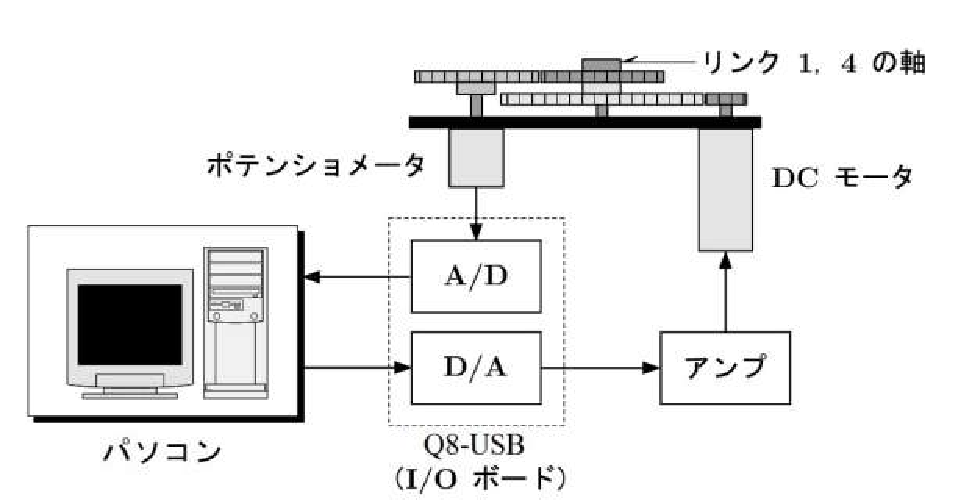
\includegraphics[width=0.8\linewidth]{figure/actuator_sensor.pdf}
    \caption{アクチュエータ(DCモータ)とセンサ(ポテンショメータ)}
    \label{fig:actuator_sensor}
\end{figure}

図\ref{fig:actuator_sensor}に示すように,2軸ロボット実験装置はリンク1,リンク4がギアを介してDCモータにより回転するようになっている.
DCモータを駆動させるためにパソコンにより計算された指令電圧は,I/OボードQ8-USBでD/A変換された後,アンプを介してDCモータに入力される.
また,リンク1,リンク4の回転角は角度センサであるポテンショメータにより電圧値として検出され,I/OボードQ8-USBでA/D変換された後,パソコンに取り込まれている.

\subsubsection{D/A変換とアクチュエータの動作確認}
\subsubsection{実験装置のセッティングと\textbf{MATLAB}/Simulinkの起動}

図\ref{fig:experiment_setup}に示すように,実験装置の2つの軸にそれぞれリンクを取り付ける.
また,図\ref{fig:terminal_connection}のようにターミナル,Universal Power Module,2軸ロボットのケーブルが接続されていることを確認する.
ただし,左側のDCモータおよびポテンショメータに対するチャネルを\textbf{CH0}(チャネル0),
右側のDCモータおよびポテンショメータに対するチャネルを\textbf{CH1}(チャネル1)とする.


\begin{figure}[H]
    \centering
    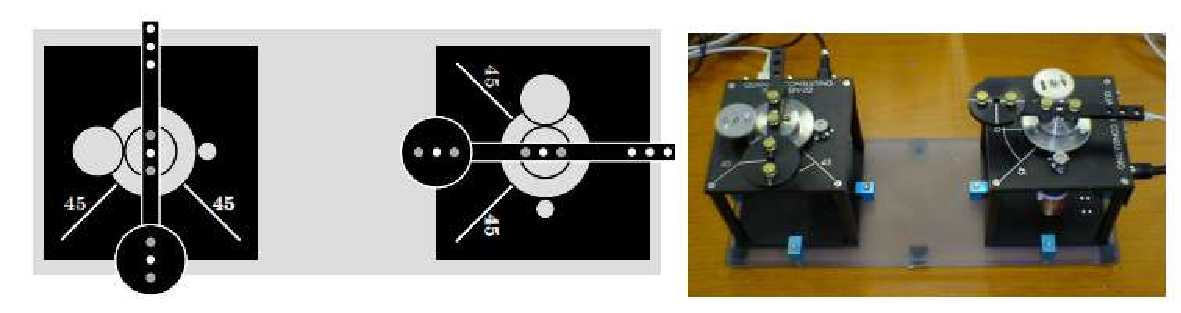
\includegraphics[width=0.8\linewidth]{figure/experiment_setup.pdf}
    \caption{実験装置}
    \label{fig:experiment_setup}
\end{figure}

\begin{figure}[H]
    \centering
    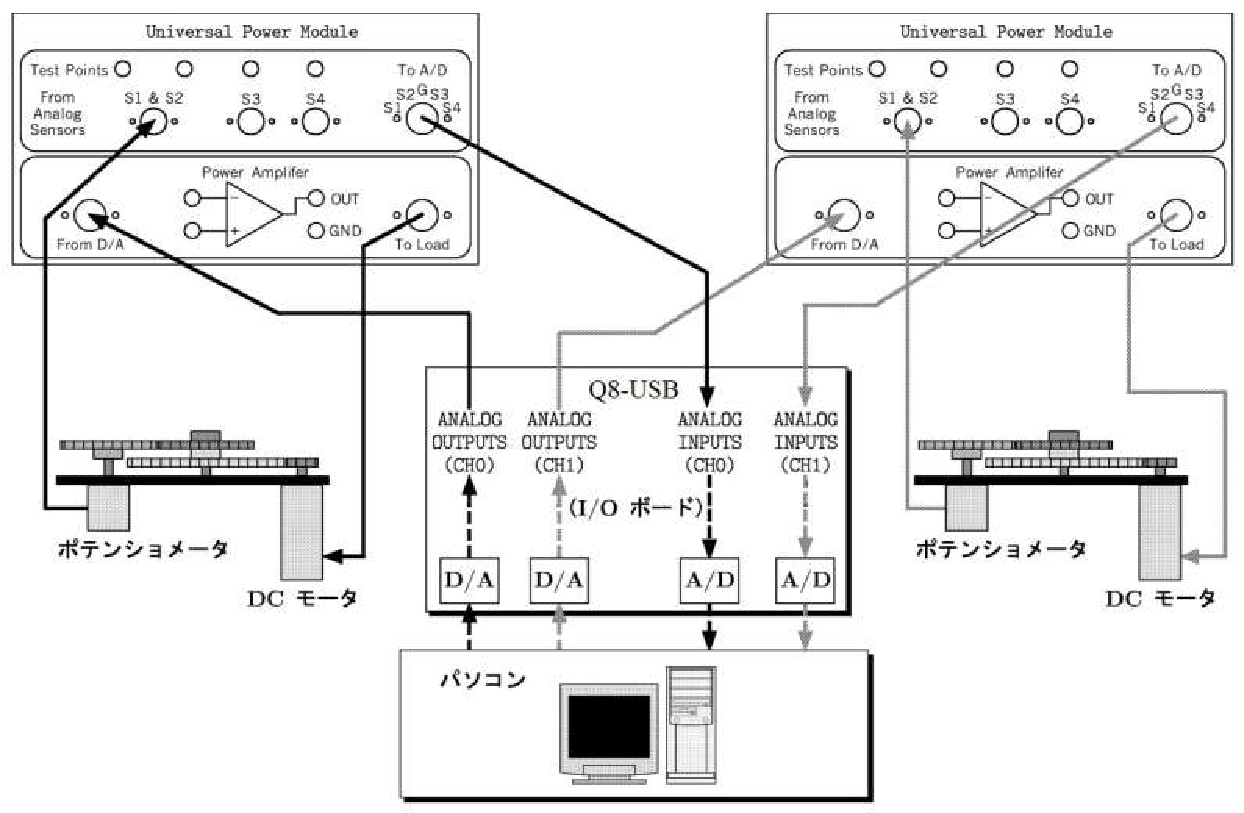
\includegraphics[width=0.95\linewidth]{figure/terminal_connection.pdf}
    \caption{実験装置の接続}
    \label{fig:terminal_connection}
\end{figure}

つぎに,Windowsスタートメニューより MATLAB R2013a を起動する.MATLAB のコマンドウィンドウ上で以下のように入力し,カレントディレクトリ(作業するフォルダ)を変更する.(Xは自分の班名に置き換える.)

\begin{tcolorbox}[colback=white,colframe=black]
    \verb|cd D:\student_senkouka\group_X|
    \end{tcolorbox}

    \subsubsection{モデルの移動と結線}

    左右のDCモータに2\,[V]の電圧を加えたときのリンクの動きを調べてみよう。
    MATLABの“現在のフォルダー”にある,“da”フォルダーを選択し,“da\_conv.slx”をダブルクリックしてSimulinkモデルを起動する。
    起動したモデルを図\ref{fig:da_conv}のように結線する。
    また,各ブロックをダブルクリックして,パラメータを変更する。
    

    \begin{figure}[H]
        \centering
        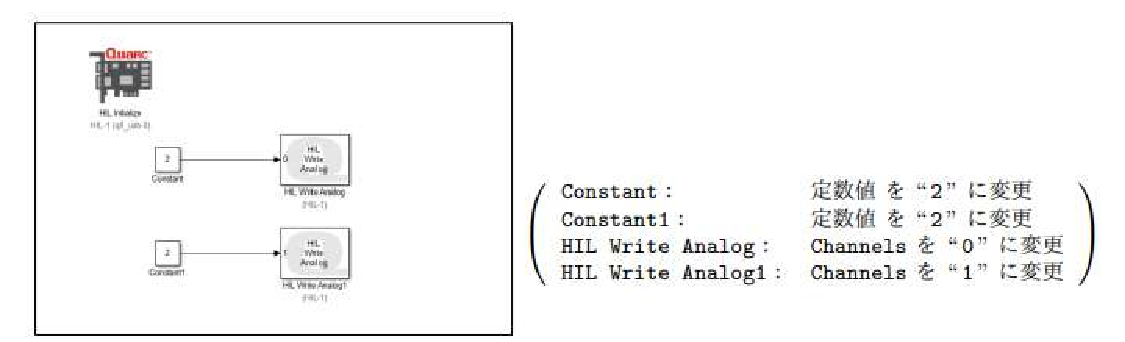
\includegraphics[width=0.9\linewidth]{figure/da_conv.pdf}
        \caption{da\_conv.slx}
        \label{fig:da_conv}
    \end{figure}
    
    \subsubsection{Simulation Parameters のパラメータ設定}

    Simulink モデルウィンドウのツールバーから``モデルコンフィグレーションパラメーター''を選択し,
    ``ソルバー''を選択,図 \ref{fig:sim_param} のようにパラメータを設定する.
    
    \begin{figure}[H]
        \centering
        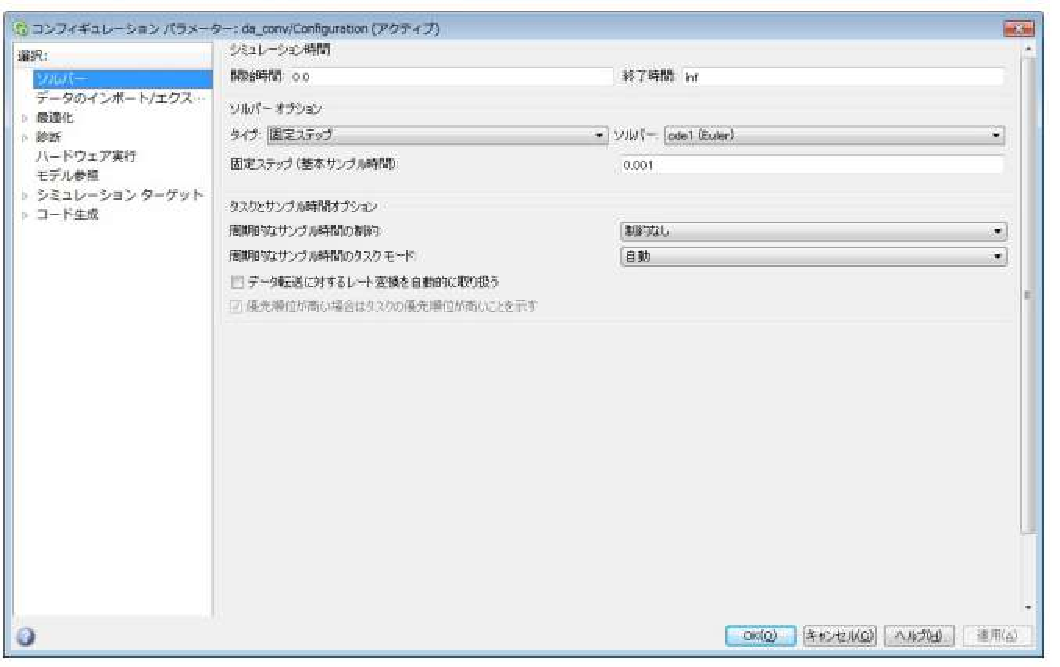
\includegraphics[width=0.8\linewidth]{figure/sim_param.pdf}
        \caption{Simulation Parameters のパラメータ設定}
        \label{fig:sim_param}
    \end{figure}
    
    \subsubsection{コンパイル}
    Dドライブのディレクトリ(フォルダ)D:\textbackslash student\_senkouka\textbackslash group\_X\textbackslash 
    da(Xは自分の班名)がカレントディレクトリとなっているかどうか確かめる.
    カレントディレクトリとなっていない場合は現在のフォルダーを操作してカレントディレクトリを変更する.
    
    \begin{figure}[H]
        \centering
        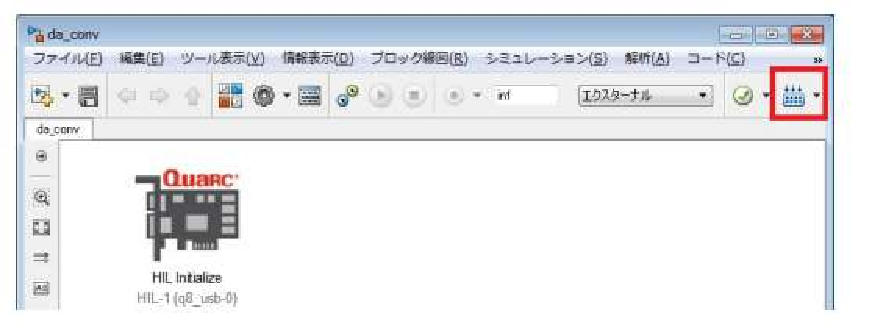
\includegraphics[width=0.8\linewidth]{figure/compile_button.pdf}
        \caption{コンパイル}
        \label{fig:compile_button}
    \end{figure}
    
    つぎに,“da\_conv.slx” をコンパイルするためには,図~\ref{fig:compile_button} に示すように Simulink モデルのツールバーの右端にあるアイコンをクリック,モデルのビルドを選択すればよい.別の方法としては Simulink モデルのメニューから「QUARC/Build」を選択しても良い.このとき,エラーがなければ MATLAB Command Window に以下のようなメッセージが表示され,コンパイルが終了する.
\footnotesize
\begin{verbatim}
### コードをビルドフォルダーに生成しています: D:\student_senkouka\group_xx\da\da_conv_quarc_win64
### Invoking Target Language Compiler on da_conv.rtw
### Using System Target File: C:\Program Files\Quanser\QUARC\quarc_win64.tlc
### Loading TLC function libraries
.....................《略》 .....................
### Created executable da_conv.rtw-win64
### Downloading da_conv to target ’shmem://quarc-target:1’ ...
### Model da_conv has been downloaded to target ’shmem://quarc-target:1’
\end{verbatim}

        \subsubsection{実験}

        コンパイル終了後,図~\ref{fig:experiment_start} に示すように Simulink モデルのツールバーで “ターゲットに接続” アイコンをクリックし,
        その右のアイコンの “実行” をクリックすると,モータドライバに一定の電圧 2~[V] が加わり,
        リンクが一定速度で時計回りに回転することが確認できる.停止させる場合には “実行” アイコンの右にある “停止” アイコンをクリックすればよい.
        実行の方法として,Simulink モデルのメニューから「QUARC/Start」を選択しても実行ができる.
        また停止方法として Simulink モデルのメニューから「QUARC/Stop」を選択してもよい.
        
        \begin{figure}[H]
            \centering
            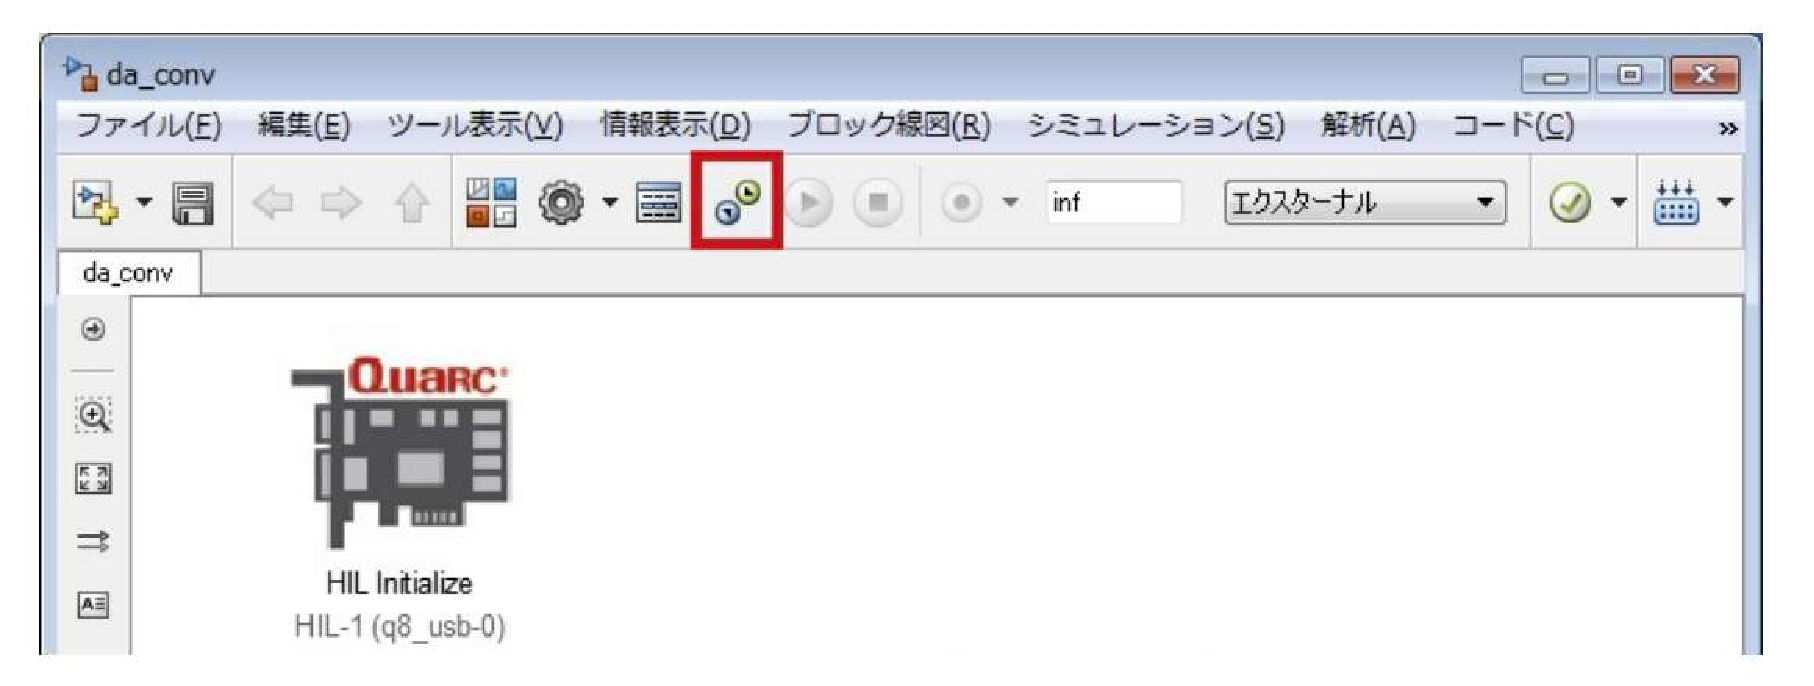
\includegraphics[width=0.85\linewidth]{figure/experiment_start.pdf}
            \caption{実機実験の開始}
            \label{fig:experiment_start}
        \end{figure}
        
        \subsubsection{A/D 変換とセンサの動作確認}

        本実験装置では,角度センサにポテンショメータを用いている.このポテンショメータは軸の回転角に比例した電圧 $-5 \sim +5$~[V] をアナログ信号として出力し,
        また,この電圧と軸の回転角との関係は,$1$~[V] あたり $-35$~[deg] である.
        
        ポテンショメータの動作確認をするために,図~\ref{fig:ad_conv_model} の実機実験モデル “\texttt{ad\_conv.slx}” を作成する.
        
        \begin{figure}[H]
            \centering
            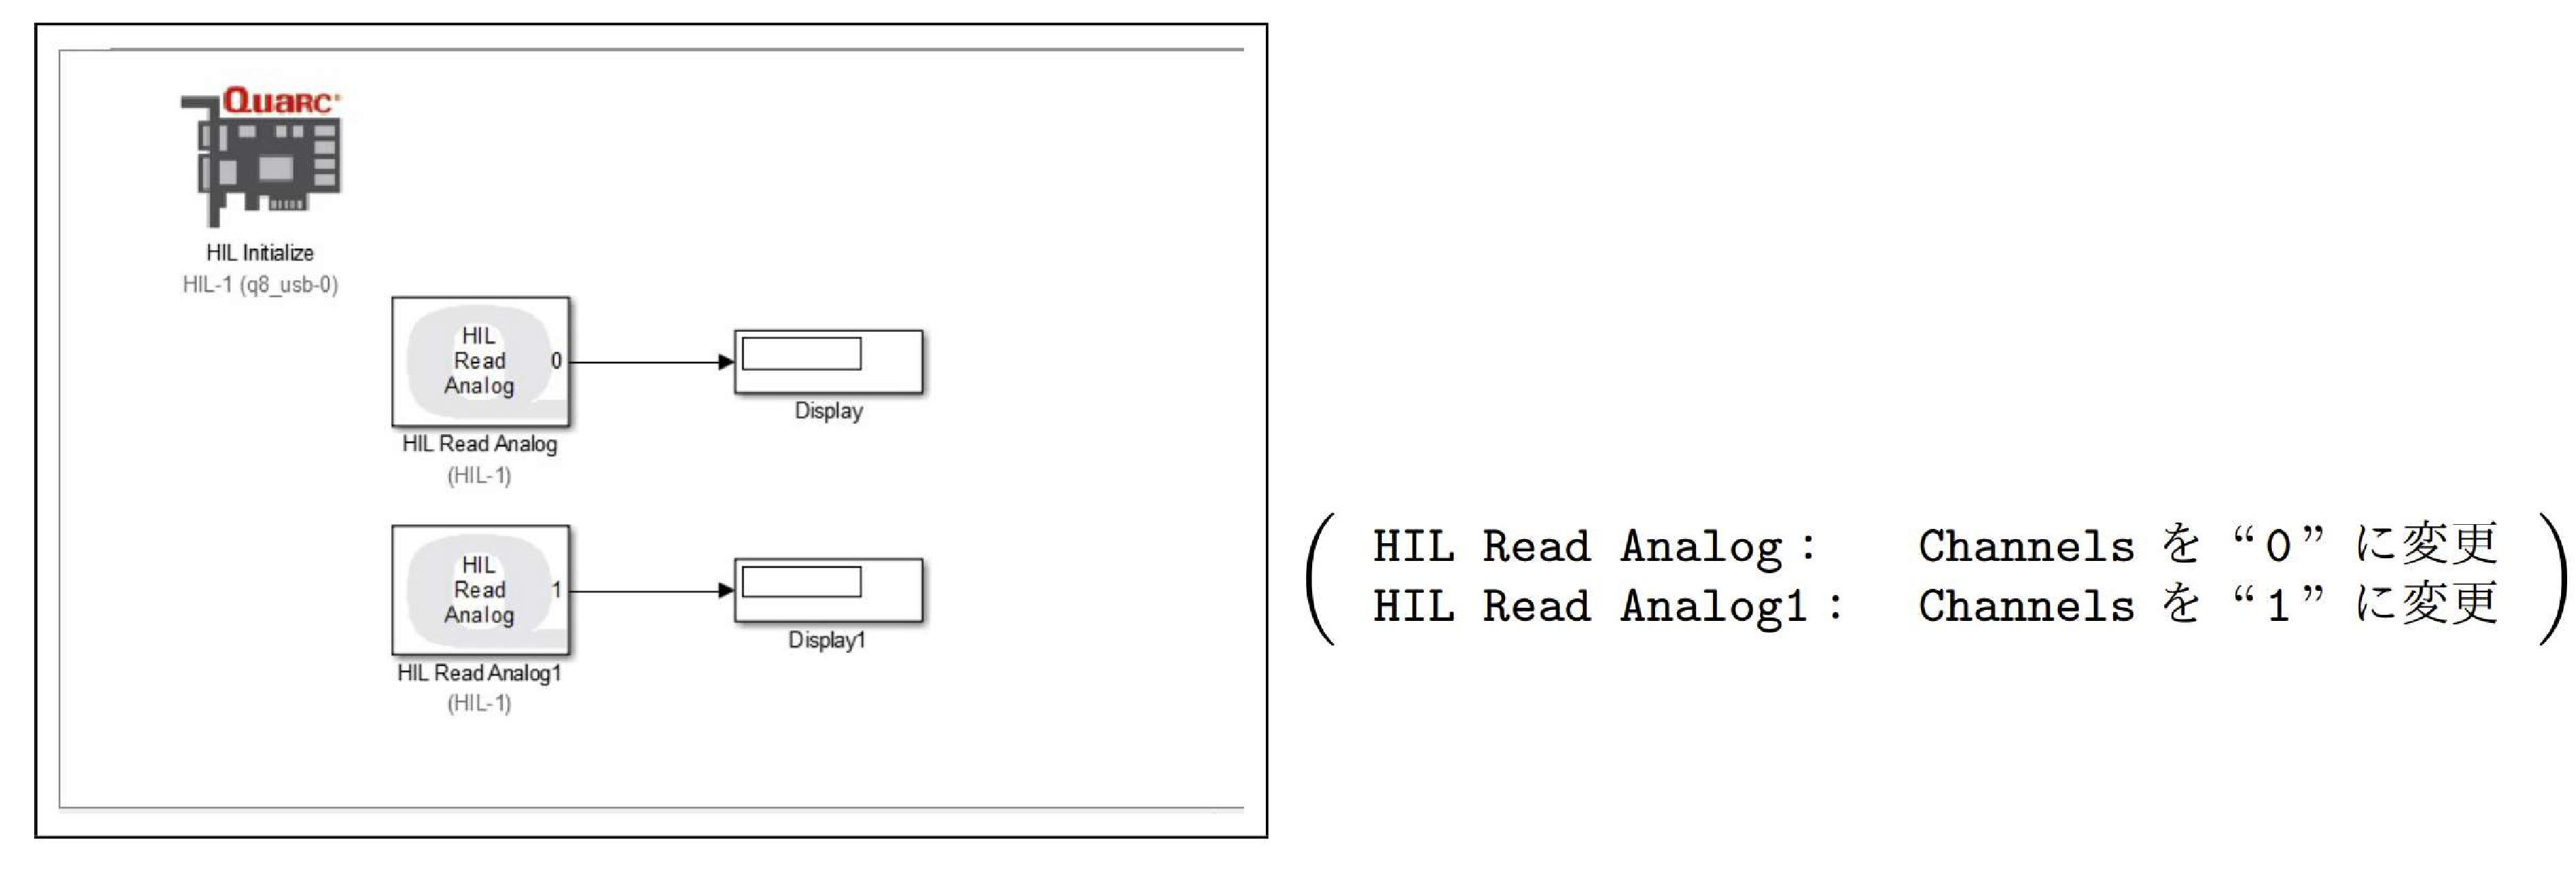
\includegraphics[width=0.9\linewidth]{figure/ad_conv_model.pdf}
            \caption{“\texttt{ad\_conv.slx}”}
            \label{fig:ad_conv_model}
        \end{figure}
        
        つぎに,図~\ref{fig:parameter_setting} で示したようにパラメータ設定を行い,図~\ref{fig:compile_adconv} 節で示したように “\texttt{ad\_conv.slx}” をコンパイルする.

        以上の準備の下,リンクを図~\ref{fig:adconv_run_start}~(a) の状態にして,“Start” アイコンをクリックすると,センサからの電圧が図~\ref{fig:voltage_0V}~(a) のように $0$~[V] 程度であることが確認できる.
        
        先に述べたように,本実験装置で用いているポテンショメータは,$1$~[V] あたり $-35$~[deg]($= -0.6109$~[rad])であるから,リンクを反時計回りに $45$~[deg] $= \pi/4$~[rad] 回転させると $-1.2857$~[V] の電圧が発生するはずである.
        
        実際,リンクを図~\ref{fig:adconv_run_start}~(b) のように反時計回りに $45$~[deg] 回転させると,センサからの電圧が図~\ref{fig:voltage_-1.2857V}~(b) のように $-1.2857$~[V] 程度であることが確認できる.



% 図3.9
\begin{figure}[htbp]
    \centering
    \begin{subfigure}[b]{0.45\linewidth}
        \centering
        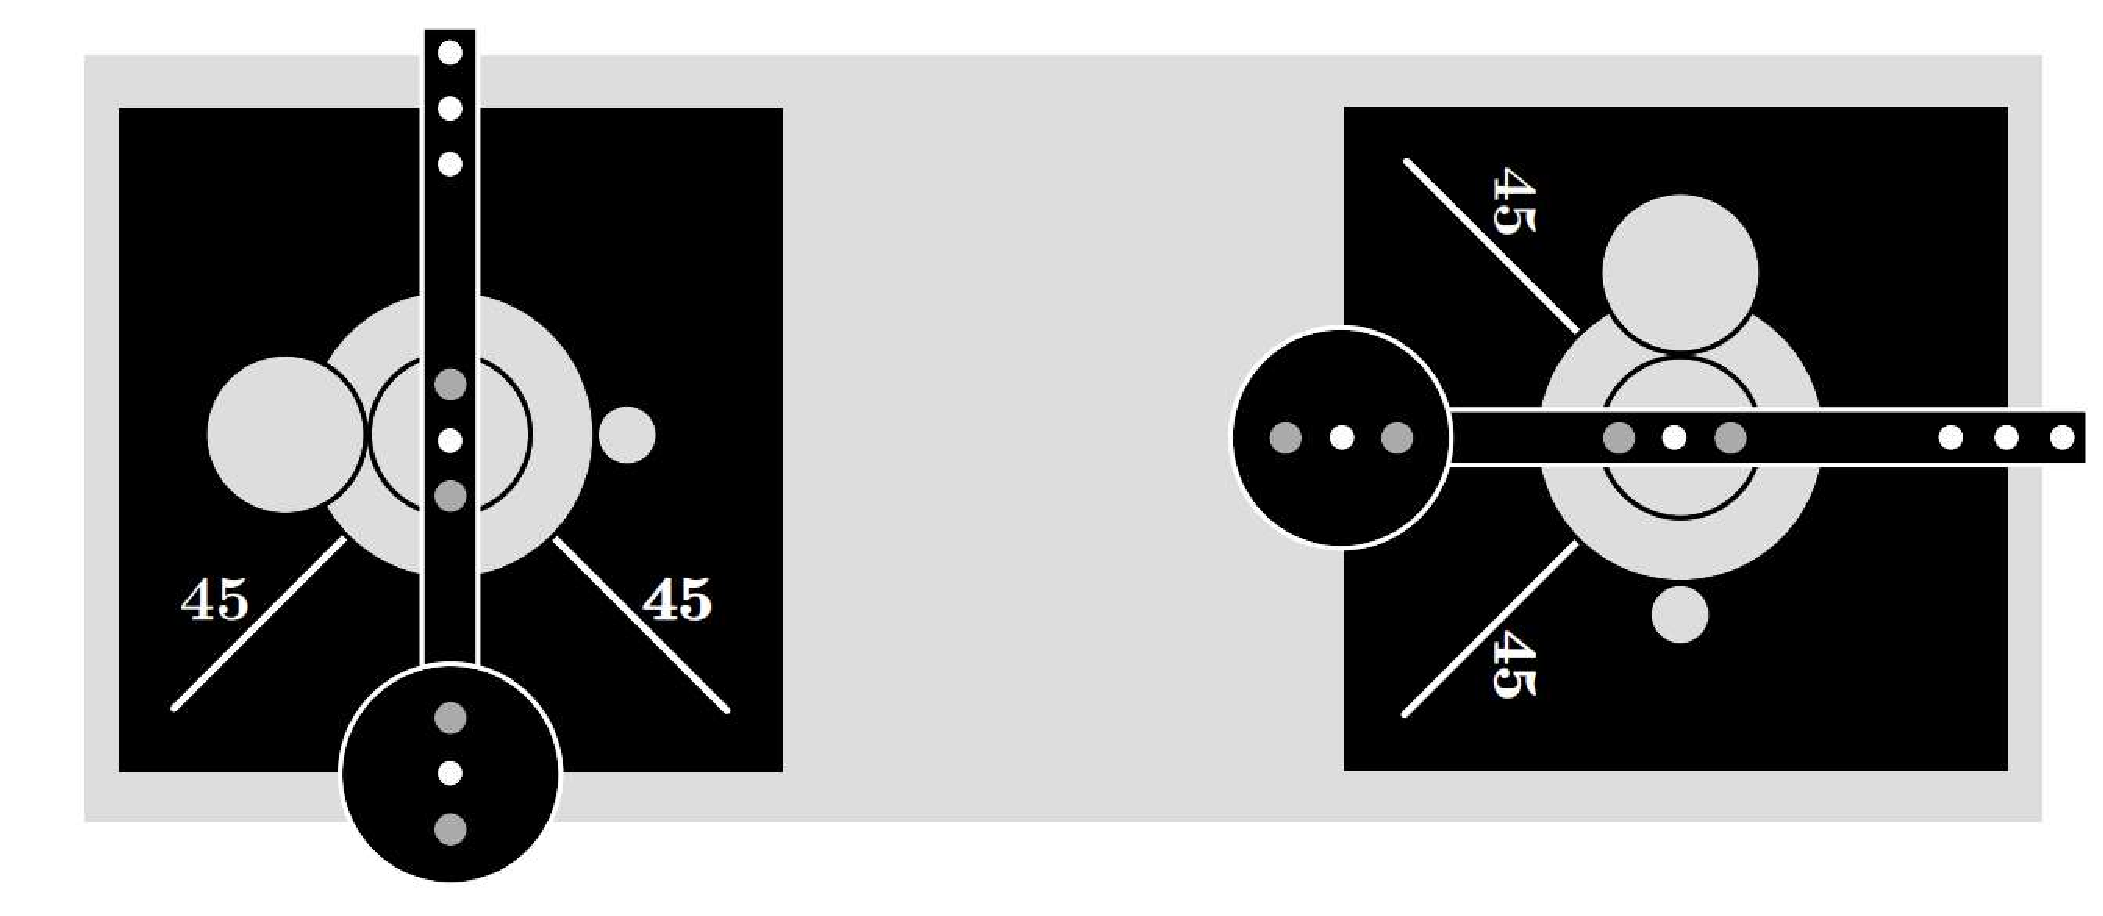
\includegraphics[width=\linewidth]{figure/link_0deg.pdf}
        \caption{初期状態}
    \end{subfigure}
    \hfill
    \begin{subfigure}[b]{0.45\linewidth}
        \centering
        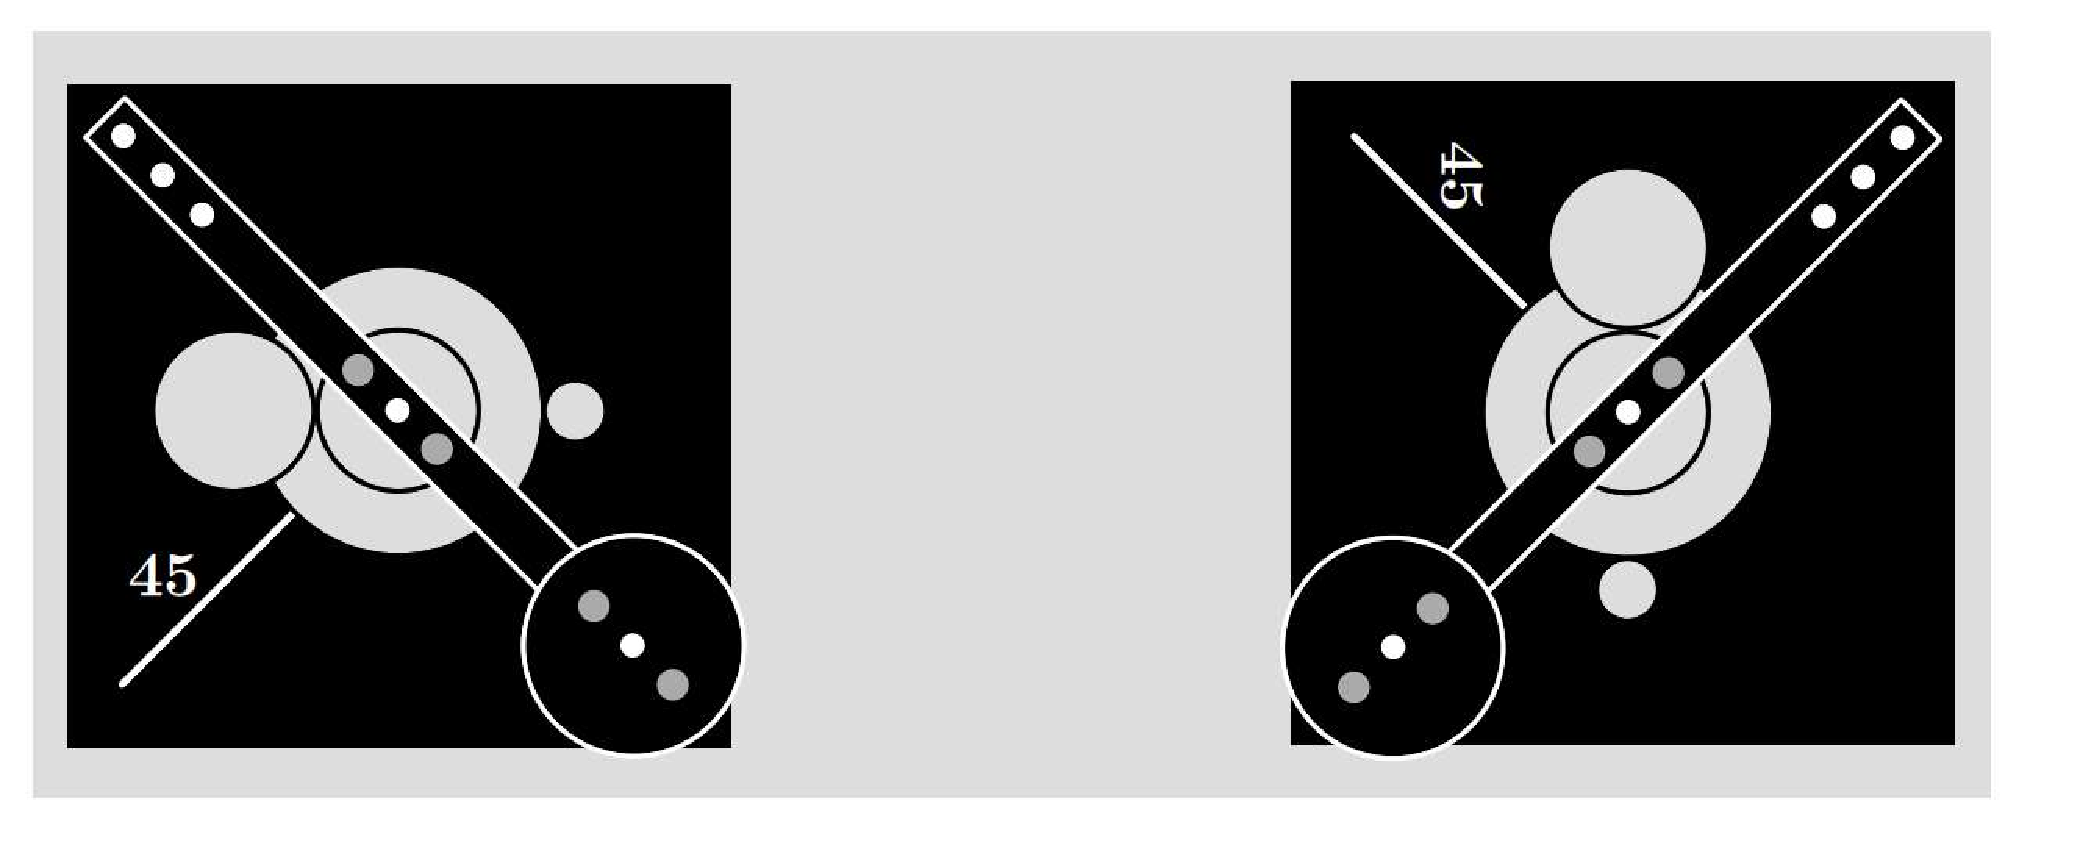
\includegraphics[width=\linewidth]{figure/link_45deg.pdf}
        \caption{リンクを反時計回りに $45$~[deg] 回転させた状態}
    \end{subfigure}
    \caption{リンクを手で反時計回りに $45$~[deg] 回転させた状態}
    \label{fig:adconv_run_start}
\end{figure}

% 図3.10
\begin{figure}[htbp]
    \centering
    \begin{subfigure}[b]{0.45\linewidth}
        \centering
        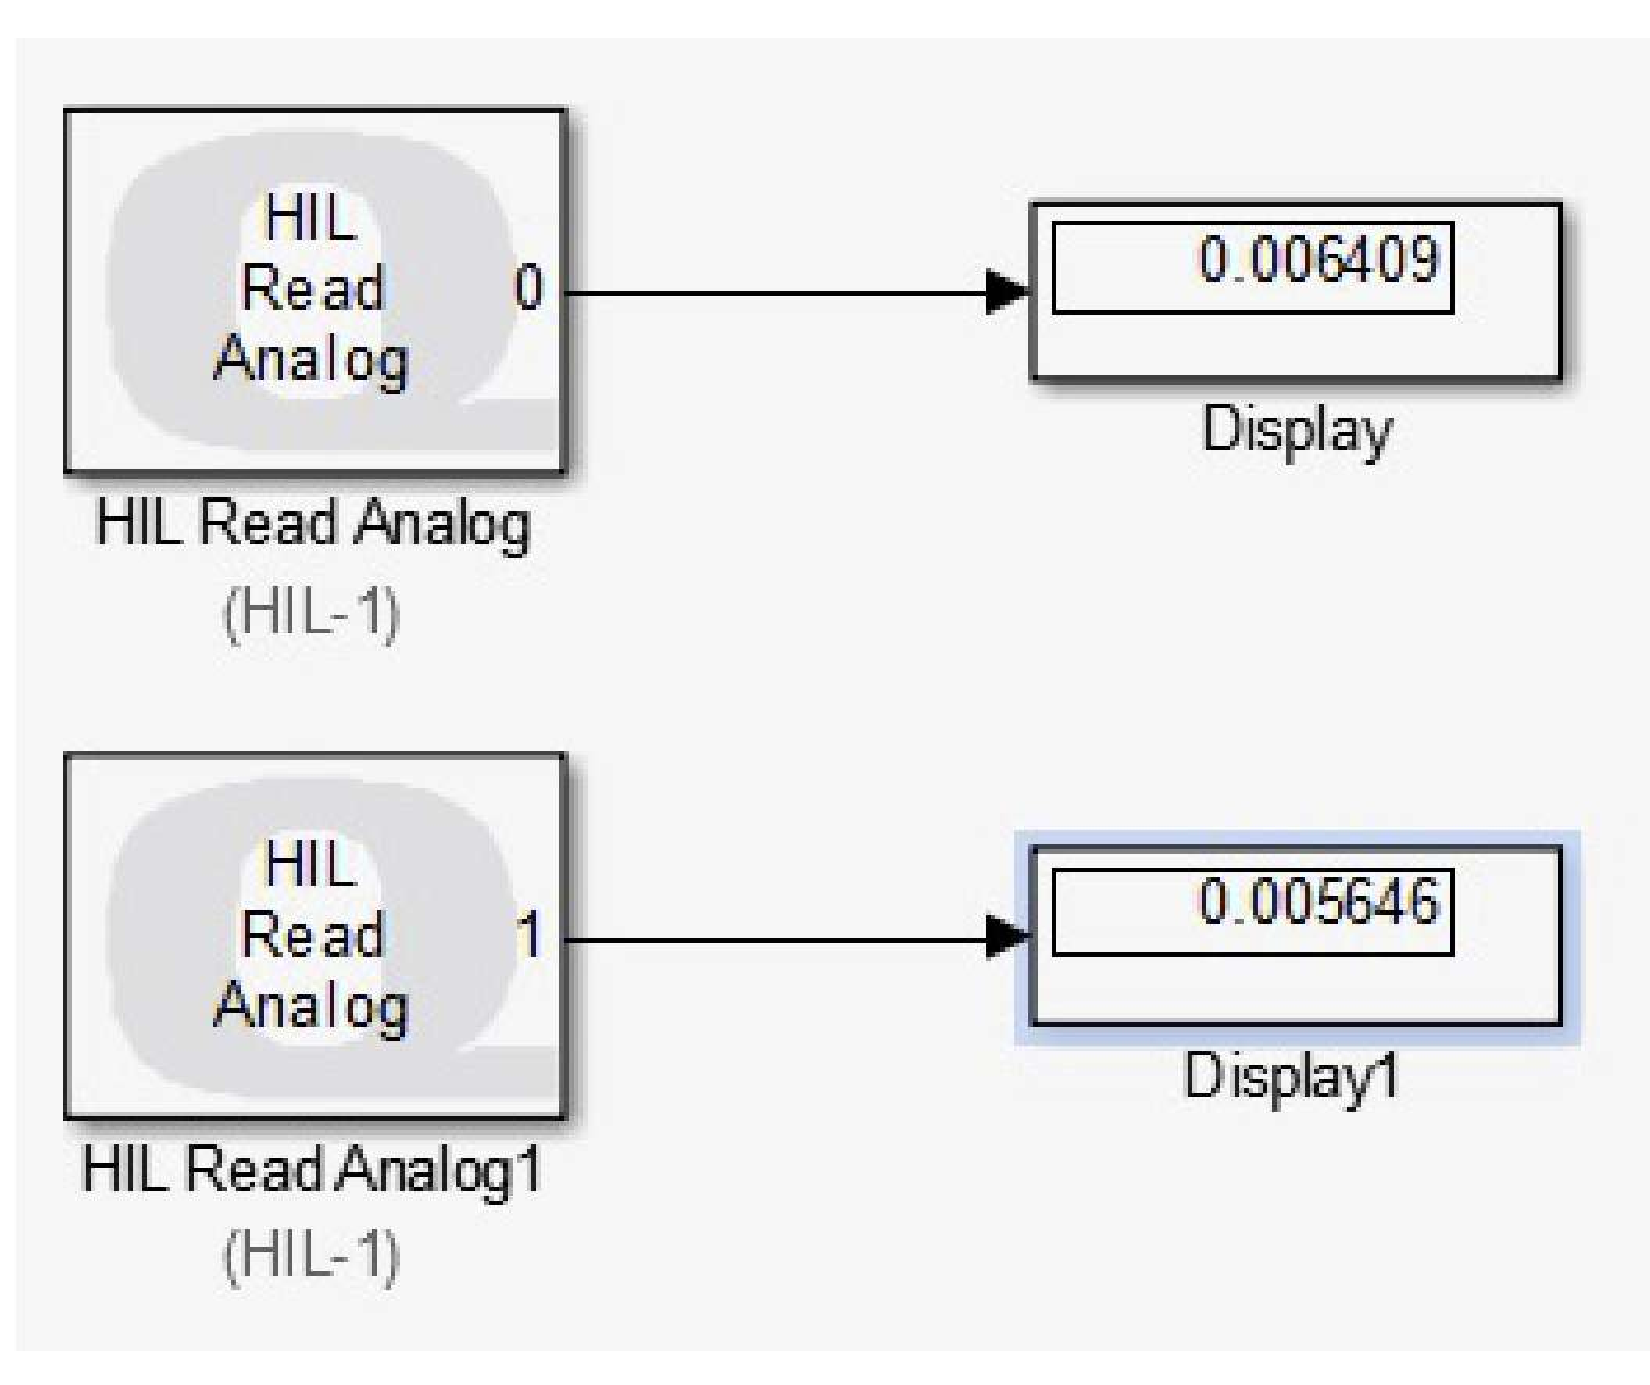
\includegraphics[width=\linewidth]{figure/voltage_before.pdf}
        \caption{初期状態}
        \label{fig:voltage_0V}
    \end{subfigure}
    \hfill
    \begin{subfigure}[b]{0.45\linewidth}
        \centering
        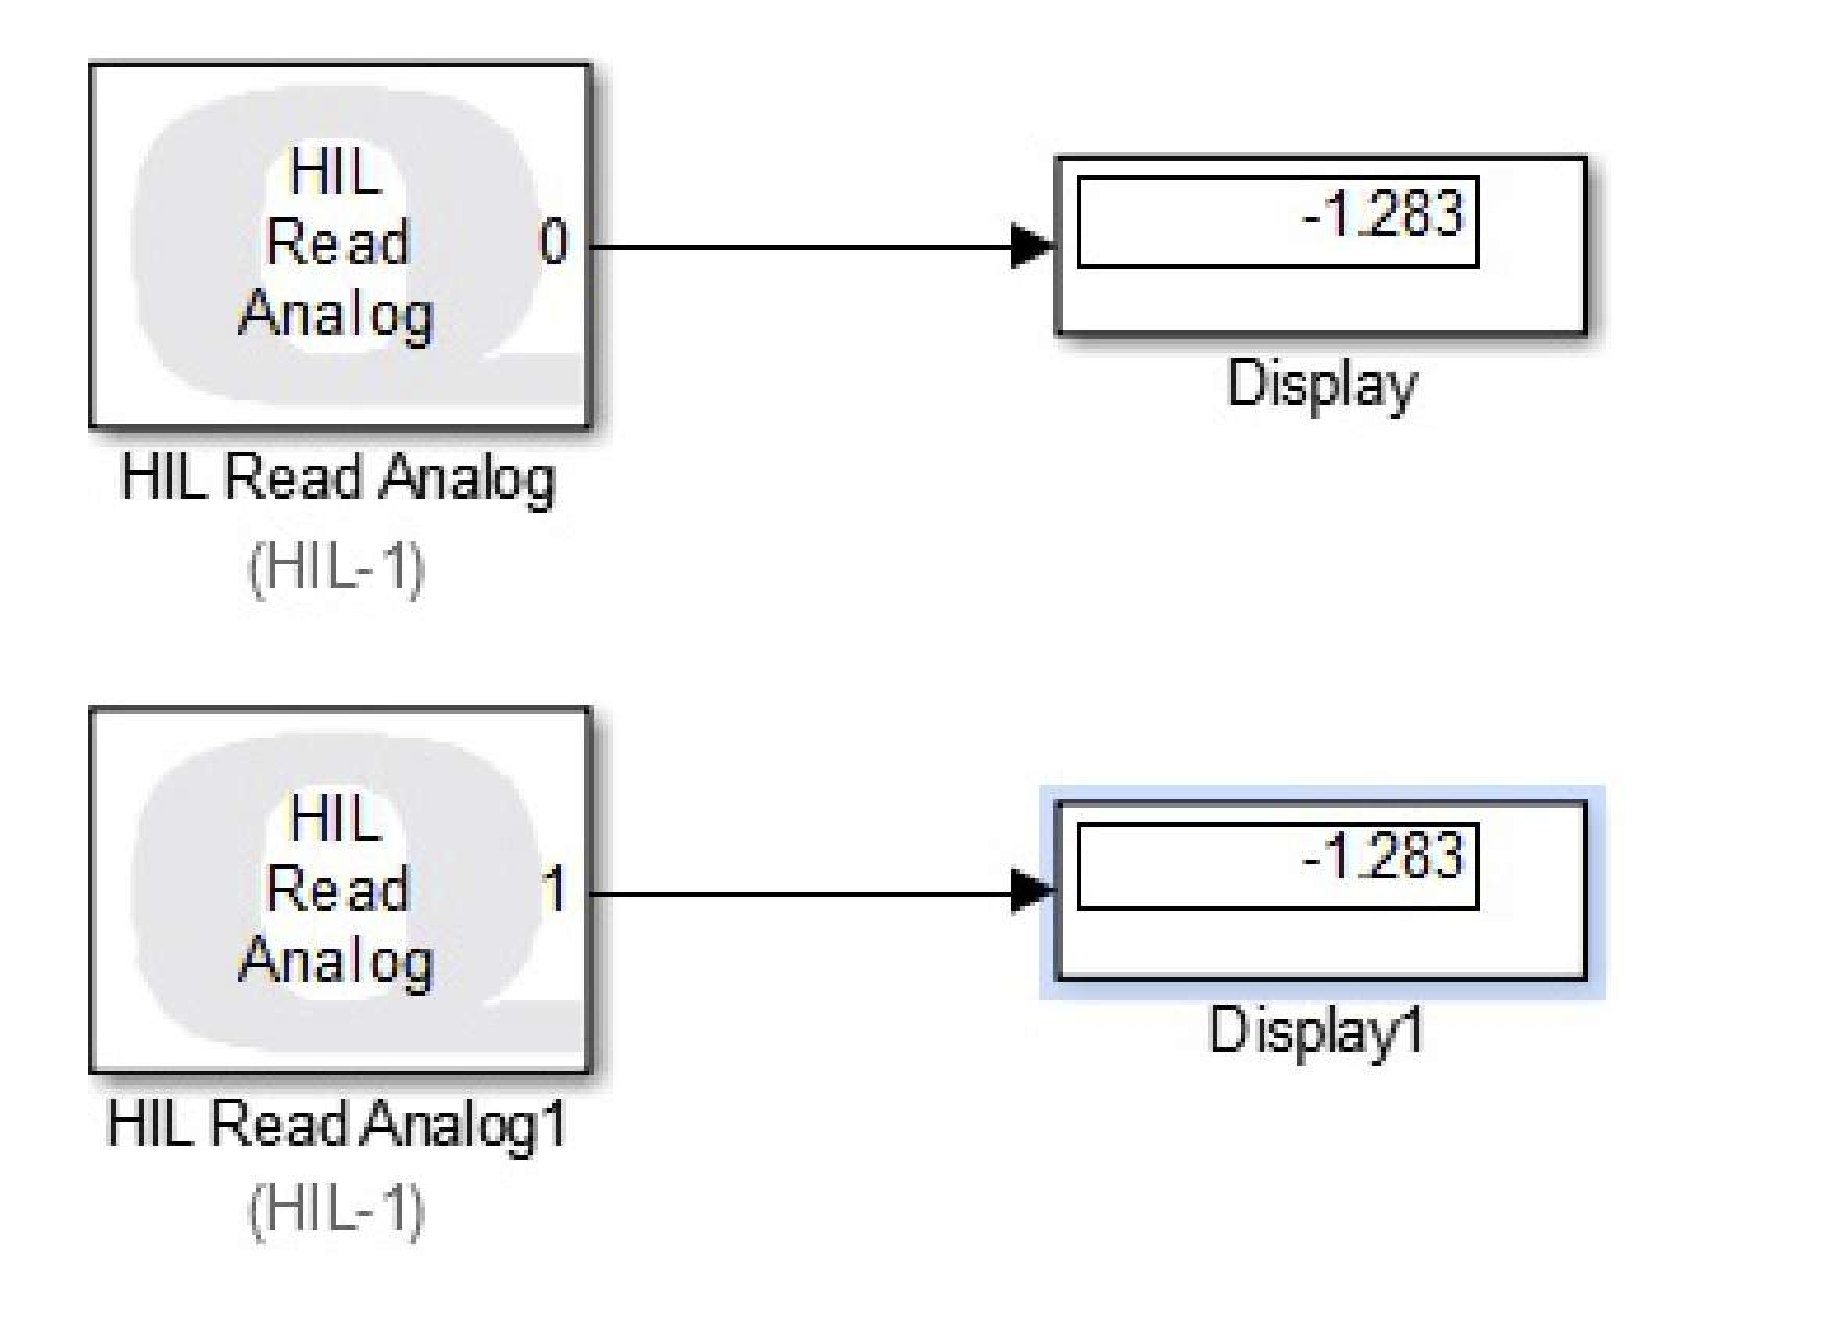
\includegraphics[width=\linewidth]{figure/voltage_after.pdf}
        \caption{リンクを反時計回りに $45$~[deg] 回転させた状態}
        \label{fig:voltage_-1.2857V}
    \end{subfigure}
    \caption{リンクを手で反時計回りに $45$~[deg] 回転させたときの出力電圧}
    \label{fig:output_voltage_change}
\end{figure}

\subsection{実験結果}
\subsubsection{D/A変換とアクチュエータの動作確認}
図~\ref{fig:response_under_constant_voltage} に示すように,DCモータに $2$~[V] の電圧を加えると,リンクが時計回りに回転し,リンクの角度 $\theta_{x}(t)$,$\theta_{y}(t)$ が弧度法の単位~[rad] で得られることが確認できた.

\subsubsection{A/D変換とセンサの動作確認}
図~\ref{fig:output_voltage_change} に示すように,リンクを反時計回りに $45$~[deg] 回転させたとき,センサからの電圧が $-1.2857$~[V] 程度であることが確認できた.

\subsection{考察}
アクチュエータの動作確認では,正の電圧をDCモータに加えるとリンクが時計回りに回転することが確認できた.また,センサの動作確認では,ポテンショメータが角度に比例した電圧を出力することが確認できた.これにより,2軸ロボットの動作が正確に制御可能であることが示された.
